\documentclass[mathserif]{beamer}

\setbeamertemplate{frametitle}[default][center]%Centers the frame title.
\setbeamertemplate{navigation symbols}{}%Removes navigation symbols.
\setbeamertemplate{footline}{\raisebox{5pt}{\makebox[\paperwidth]{\hfill\makebox[10pt]{\scriptsize\insertframenumber}}}}
\setbeamertemplate{caption}[numbered]

%\usepackage[colorlinks = true]{hyperref}

%\usepackage[colorlinks = true,
%            linkcolor = blue,
%            urlcolor  = blue,
%            citecolor = blue,
%            anchorcolor = blue]{hyperref}

%\newcommand{\tth}   {\mbox{$\theta$}}
\newcommand{\thh}   {\mbox{$\theta$}}
\newcommand{\su}   {\mbox{$\sigma^2$}}
\newcommand{\so}   {\mbox{$\sigma_0^2$}}
\newcommand{\ko}   {\mbox{$\kappa_0$}}
\newcommand{\no}   {\mbox{$\nu_0$}}
\newcommand{\mo}   {\mbox{$\mu_0$}}
\newcommand{\ti}   {\mbox{$\tilde{x}$}}
\newcommand{\la}   {\mbox{$\lambda$}}
\newcommand{\bx}   {\mbox{$\bm{x}$}}
\newcommand{\bZ}   {\mbox{$\bm{Z}$}}
\newcommand{\bX}   {\mbox{$\bm{X}$}}
\newcommand{\bY}   {\mbox{$\bm{Y}$}}
\newcommand{\bA}   {\mbox{$\bm{A}$}}
\newcommand{\ba}   {\mbox{$\bm{a}$}}
\newcommand{\bb}   {\mbox{$\bm{b}$}}
\newcommand{\bt}   {\mbox{$\bm{t}$}}
\newcommand{\bz}   {\mbox{$\bm{z}$}}
\newcommand{\bw}   {\mbox{$\bm{w}$}}
\newcommand{\bbeta}   {\mbox{$\bm{\beta}$}}

\newcommand{\be}   {\mbox{$\bm{e}$}}
\newcommand{\bu}   {\mbox{$\bm{u}$}}
\newcommand{\bv}   {\mbox{$\bm{v}$}}
\newcommand{\sig}   {\mbox{$\Sigma$}}
\newcommand{\sigx}   {\mbox{$\Sigma_{XX}$}}
\newcommand{\sigxy}   {\mbox{$\Sigma_{XY}$}}
\newcommand{\tr}   {\mbox{$\text{tr}$}}
\newcommand{\ddet}   {\mbox{$\text{det}$}}
\newcommand\independent{\protect\mathpalette{\protect\independenT}{\perp}}
\def\independenT#1#2{\mathrel{\rlap{$#1#2$}\mkern2mu{#1#2}}}

\newcommand{\Expect}[1]{\ensuremath{\mathbf{E}\left[ #1 \right]}}
%\newcommand{\Var}[1]{\ensuremath{\mathrm{Var}\left[ #1 \right]}}
%\newcommand{\Cov}[1]{\ensuremath{\mathrm{Cov}\left[ #1 \right]}}
\newcommand{\MSE}{\ensuremath{\mathrm{MSE}}}
\newcommand{\RSS}{\ensuremath{\mathrm{RSS}}}
\newcommand{\Prob}[1]{\ensuremath{\mathrm{Pr}\left( #1 \right)}}
\newcommand{\ProbEst}[1]{\ensuremath{\widehat{\mathrm{Pr}}\left( #1 \right)}}
\DeclareMathOperator*{\argmin}{argmin} % thanks, wikipedia!
\DeclareMathOperator*{\argmax}{argmax} % thanks, wikipedia!
\DeclareMathOperator*{\sgn}{sgn} % thanks, wikipedia!

\newcommand{\lam}{\lambda}
\newcommand{\bmu}{\bm{\mu}}
%\newcommand{\bx}{\ensuremath{\mathbf{X}}}
\newcommand{\X}{\ensuremath{\mathbf{X}}}
\newcommand{\w}{\ensuremath{\mathbf{w}}}
\newcommand{\h}{\ensuremath{\mathbf{h}}}
\newcommand{\V}{\ensuremath{\mathbf{V}}}
%\newcommand{\tr}{\operatorname{tr}}

%\newcommand{\bx}{\ensuremath{\mathbf{X}}}
%\newcommand{\X}{\ensuremath{\mathbf{x}}}
%\newcommand{\w}{\ensuremath{\mathbf{w}}}
%\newcommand{\h}{\ensuremath{\mathbf{h}}}
%\newcommand{\V}{\ensuremath{\mathbf{v}}}
%\newcommand{\Cov}{\text{Cov}}
%\newcommand{\Var}{\text{Var}}

\DeclareMathOperator{\var}{Var}
\DeclareMathOperator{\cov}{Cov}
\newcommand{\Var}[1]{\ensuremath{\mathrm{Var}\left[ #1 \right]}}
\newcommand{\Cov}[1]{\ensuremath{\mathrm{Cov}\left[ #1 \right]}}


\newcommand{\indep}{\rotatebox{90}{\ensuremath{\models}}}
\newcommand{\notindep}{\not\hspace{-.05in}\indep}







\usepackage{float,bm}
\floatstyle{boxed}
\newfloat{code}{tp}{code}
\floatname{code}{Code Example}
\newcommand{\tth}   {\mbox{$\theta$}}
\newcommand{\thh}   {\mbox{$\theta$}}
\newcommand{\su}   {\mbox{$\sigma^2$}}
\newcommand{\so}   {\mbox{$\sigma_0^2$}}
\newcommand{\ko}   {\mbox{$\kappa_0$}}
\newcommand{\no}   {\mbox{$\nu_0$}}
\newcommand{\mo}   {\mbox{$\mu_0$}}
\newcommand{\ti}   {\mbox{$\tilde{x}$}}
\newcommand{\la}   {\mbox{$\lambda$}}
\newcommand{\bx}   {\mbox{$\bm{x}$}}
\newcommand{\bZ}   {\mbox{$\bm{Z}$}}
\newcommand{\bX}   {\mbox{$\bm{X}$}}
\newcommand{\bY}   {\mbox{$\bm{Y}$}}
\newcommand{\bA}   {\mbox{$\bm{A}$}}
\newcommand{\ba}   {\mbox{$\bm{a}$}}
\newcommand{\bb}   {\mbox{$\bm{b}$}}
\newcommand{\bt}   {\mbox{$\bm{t}$}}
\newcommand{\bz}   {\mbox{$\bm{z}$}}
\newcommand{\bw}   {\mbox{$\bm{w}$}}
\newcommand{\bbeta}   {\mbox{$\bm{\beta}$}}

\newcommand{\be}   {\mbox{$\bm{e}$}}
\newcommand{\bu}   {\mbox{$\bm{u}$}}
\newcommand{\bv}   {\mbox{$\bm{v}$}}
\newcommand{\sig}   {\mbox{$\Sigma$}}
\newcommand{\sigx}   {\mbox{$\Sigma_{XX}$}}
\newcommand{\sigxy}   {\mbox{$\Sigma_{XY}$}}
\newcommand{\tr}   {\mbox{$\text{tr}$}}
\newcommand{\ddet}   {\mbox{$\text{det}$}}
\newcommand\independent{\protect\mathpalette{\protect\independenT}{\perp}}
\def\independenT#1#2{\mathrel{\rlap{$#1#2$}\mkern2mu{#1#2}}}

\newcommand{\Expect}[1]{\ensuremath{\mathbf{E}\left[ #1 \right]}}
%\newcommand{\Var}[1]{\ensuremath{\mathrm{Var}\left[ #1 \right]}}
%\newcommand{\Cov}[1]{\ensuremath{\mathrm{Cov}\left[ #1 \right]}}
\newcommand{\MSE}{\ensuremath{\mathrm{MSE}}}
\newcommand{\RSS}{\ensuremath{\mathrm{RSS}}}
\newcommand{\Prob}[1]{\ensuremath{\mathrm{Pr}\left( #1 \right)}}
\newcommand{\ProbEst}[1]{\ensuremath{\widehat{\mathrm{Pr}}\left( #1 \right)}}
\DeclareMathOperator*{\argmin}{argmin} % thanks, wikipedia!
\DeclareMathOperator*{\argmax}{argmax} % thanks, wikipedia!
\DeclareMathOperator*{\sgn}{sgn} % thanks, wikipedia!

\newcommand{\lam}{\lambda}
\newcommand{\bmu}{\bm{\mu}}
%\newcommand{\bx}{\ensuremath{\mathbf{X}}}
\newcommand{\X}{\ensuremath{\mathbf{X}}}
\newcommand{\w}{\ensuremath{\mathbf{w}}}
\newcommand{\h}{\ensuremath{\mathbf{h}}}
\newcommand{\V}{\ensuremath{\mathbf{V}}}
%\newcommand{\tr}{\operatorname{tr}}

%\newcommand{\bx}{\ensuremath{\mathbf{X}}}
%\newcommand{\X}{\ensuremath{\mathbf{x}}}
%\newcommand{\w}{\ensuremath{\mathbf{w}}}
%\newcommand{\h}{\ensuremath{\mathbf{h}}}
%\newcommand{\V}{\ensuremath{\mathbf{v}}}
%\newcommand{\Cov}{\text{Cov}}
%\newcommand{\Var}{\text{Var}}

\DeclareMathOperator{\var}{Var}
\DeclareMathOperator{\cov}{Cov}
\newcommand{\Var}[1]{\ensuremath{\mathrm{Var}\left[ #1 \right]}}
\newcommand{\Cov}[1]{\ensuremath{\mathrm{Cov}\left[ #1 \right]}}


\newcommand{\indep}{\rotatebox{90}{\ensuremath{\models}}}
\newcommand{\notindep}{\not\hspace{-.05in}\indep}






%\usepackage{fontspec}
%\setmainfont{Tahoma}

\newcommand{\del}   {\mbox{$\delta(x)$}}

%\newcommand{\lam}{\lambda}
%\newcommand{\bmu}{\bm{\mu}}
%%\newcommand{\bx}{\ensuremath{\mathbf{X}}}
%\newcommand{\X}{\ensuremath{\mathbf{x}}}
%\newcommand{\w}{\ensuremath{\mathbf{w}}}
%\newcommand{\h}{\ensuremath{\mathbf{h}}}
%\newcommand{\V}{\ensuremath{\mathbf{v}}}
%\newcommand{\cov}{\text{Cov}}
%\newcommand{\var{\text{Var}}}

%\DeclareMathOperator{\var}{Var}
%\DeclareMathOperator{\cov}{Cov}

%\newcommand{\indep}{\rotatebox{90}{\ensuremath{\models}}}
%\newcommand{\notindep}{\not\hspace{-.05in}\indep}

%\newcommand{\bX}   {\mbox{$\bm{X}$}}
%\newcommand{\bx}   {\mbox{$\bm{x}$}}
%\newcommand{\V}   {\mbox{\text{Var}}}
%\newcommand{\tth}   {\mbox{$\theta$}}
%\newcommand{\su}   {\mbox{$\sigma^2$}}
%\newcommand{\so}   {\mbox{$\sigma_0^2$}}
%\newcommand{\ko}   {\mbox{$\kappa_0$}}
%\newcommand{\no}   {\mbox{$\nu_0$}}
%\newcommand{\mo}   {\mbox{$\mu_0$}}
%\newcommand{\ti}   {\mbox{$\tilde{x}$}}
%\newcommand{\la}   {\mbox{$\lambda$}}

\newtheoremstyle{example}
{\topsep} % space above
{\topsep} % space below
{} % body font
{} % indent
{\bf} % head font
{:} % punctuation between head and body
{0.5em} % space after head
{} % manually specify head
%{\thmname{#1}\thmnumber{ #2}\thmnote{:#3}} % manually specify head



\newtheoremstyle{definition}
{\topsep} % space above
{\topsep} % space below
{} % body font
{} % indent
{\bf} % head font
{:} % punctuation between head and body
{0.5em} % space after head
{} % manually specify head
%{\thmname{#1}\thmnumber{ #2}\thmnote{:#3}} % manually specify head

\newtheoremstyle{algorithm}
{\topsep} % space above
{\topsep} % space below
{} % body font
{} % indent
{\bf} % head font
{:} % punctuation between head and body
{0.5em} % space after head
{} % manually specify head
%{\thmname{#1}\thmnumber{ #2}\thmnote{:#3}} % manually specify head



\newtheoremstyle{theorem}
{\topsep} % space above
{\topsep} % space below
{} % body font
{} % indent
{\bf} % head font
{:} % punctuation between head and body
{0.5em} % space after head
{} % manually specify head
%{\thmname{#1}\thmnumber{ #2}\thmnote{:#3}} % manually specify head




\usepackage{graphicx} %The mode "LaTeX => PDF" allows the following formats: .jpg  .png  .pdf  .mps
\graphicspath{{./PresentationPictures/}} %Where the figures folder is located
\usepackage{listings}
\usepackage{media9}
\usepackage{movie15}
\addmediapath{./Movies/}

\newcommand{\beginbackup}{
   \newcounter{framenumbervorappendix}
   \setcounter{framenumbervorappendix}{\value{framenumber}}
}
\newcommand{\backupend}{
   \addtocounter{framenumbervorappendix}{-\value{framenumber}}
   \addtocounter{framenumber}{\value{framenumbervorappendix}} 
}


%\usepackage{algorithm2e}
\usepackage[ruled,lined]{algorithm2e}
\def\algorithmautorefname{Algorithm}
\SetKwIF{If}{ElseIf}{Else}{if}{then}{else if}{else}{endif}
%\usepackage{times}
%\usepackage[tbtags]{amsmath}
%\usepackage{amssymb}
\usepackage{amsfonts}
%\usepackage{slfortheorems}
\usepackage{epsfig}
\usepackage{graphicx}
\usepackage[small]{caption}
%\usepackage[square]{natbib}
%\newcommand{\newblock}{}
%\bibpunct{(}{)}{;}{a}{}{,}
%\bibliographystyle{ims}
%\usepackage[letterpaper]{geometry}
\usepackage{color}
\setlength{\parindent}{0pt}

\usepackage{natbib}
\bibpunct{(}{)}{;}{a}{}{,}
%\usepackage{hyperref}



%\usepackage{zref-savepos}
%
%\newcounter{restofframe}
%\newsavebox{\restofframebox}
%\newlength{\mylowermargin}
%\setlength{\mylowermargin}{2pt}
%
%\newenvironment{restofframe}{%
%    \par%\centering
%    \stepcounter{restofframe}%
%    \zsavepos{restofframe-\arabic{restofframe}-begin}%
%    \begin{lrbox}{\restofframebox}%
%}{%
%    \end{lrbox}%
%    \setkeys{Gin}{keepaspectratio}%
%    \raisebox{\dimexpr-\height+\ht\strutbox\relax}[0pt][0pt]{%
%    \resizebox*{!}{\dimexpr\zposy{restofframe-\arabic{restofframe}-begin}sp-\zposy{restofframe-\arabic{restofframe}-end}sp-\mylowermargin\relax}%
%        {\usebox{\restofframebox}}%
%    }%
%    \vskip0pt plus 1filll\relax
%    \mbox{\zsavepos{restofframe-\arabic{restofframe}-end}}%
%    \par
%}


\usepackage{tikz}
\usetikzlibrary{arrows}

%\usepackage[usenames,dvipsnames]{xcolor}
\usepackage{tkz-berge}
\usetikzlibrary{fit,shapes}

\usepackage{calc}
%%
%% The tikz package is used for doing the actual drawing.
%\usepackage{tikz}
%%
%% In order to be able to put arrowheads in the middle of directed edges, we need an extra library.
\usetikzlibrary{decorations.markings}
%%
%% The next line says how the "vertex" style of nodes should look: drawn as small circles.
\tikzstyle{vertex}=[circle, draw, inner sep=0pt, minimum size=6pt]
%%
%% Next, we make a \vertex command as a shorthand in place of \node[vertex} to get that style.
\newcommand{\vertex}{\node[vertex]}
%%
%% Finally, we declare a "counter", which is what LaTeX calls an integer variable, for use in
%% the calculations of angles for evenly spacing vertices in circular arrangements.
\newcounter{Angle}

\newtheoremstyle{example}
{\topsep} % space above
{\topsep} % space below
{} % body font
{} % indent
{\bf} % head font
{:} % punctuation between head and body
{0.5em} % space after head
{} % manually specify head
%{\thmname{#1}\thmnumber{ #2}\thmnote{:#3}} % manually specify head

\theoremstyle{example}
\newtheorem{ex}{Example}[section]

\newtheoremstyle{definition}
{\topsep} % space above
{\topsep} % space below
{} % body font
{} % indent
{\sc} % head font
{:} % punctuation between head and body
{0.5em} % space after head
{} % manually specify head
%{\thmname{#1}\thmnumber{ #2}\thmnote{:#3}} % manually specify head

\theoremstyle{definition}
\newtheorem{defn}{Definition}[section]

\theoremstyle{rem}
\newtheorem{rem}{Remark}[section]

\newtheoremstyle{theorem}
{\topsep} % space above
{\topsep} % space below
{} % body font
{} % indent
{\sc} % head font
{:} % punctuation between head and body
{0.5em} % space after head
{} % manually specify head
%{\thmname{#1}\thmnumber{ #2}\thmnote{:#3}} % manually specify head

\theoremstyle{theorm}
\newtheorem{thm}{Theorem}[section]



%%%to add in new counter for slides in beamer

%\setbeamertemplate{footline}{
%  \leavevmode%
%  \hbox{%
%  \begin{beamercolorbox}[wd=.333333\paperwidth,ht=2.25ex,dp=1ex,center]{author in head/foot}%
%    \usebeamerfont{author in head/foot}\insertshortauthor~~(\insertshortinstitute)
%  \end{beamercolorbox}%
%  \begin{beamercolorbox}[wd=.333333\paperwidth,ht=2.25ex,dp=1ex,center]{title in head/foot}%
%    \usebeamerfont{title in head/foot}\insertshorttitle
%  \end{beamercolorbox}%
%  \begin{beamercolorbox}[wd=.333333\paperwidth,ht=2.25ex,dp=1ex,right]{date in head/foot}%
%    \usebeamerfont{date in head/foot}\insertshortdate{}\hspace*{2em}
%    \insertframenumber{} \hspace*{2ex} % hier hat's sich ge�ndert
%  \end{beamercolorbox}}%
%  \vskip0pt%
%}



%%%%%

\newcommand*\oldmacro{}
\let\oldmacro\insertshortauthor
\renewcommand*\insertshortauthor{
  \leftskip=.3cm
\insertframenumber\,/\,\inserttotalframenumber\hfill\oldmacro}




%\excludecomment{notbeamer}
%\includecomment{beamer}



\title{Noninformative (``Default") Bayes:\\ A Quick Review}
\author{Rebecca C. Steorts \\ Bayesian Methods and Modern Statistics: STA 360/601}
\date{Lecture 7}

\begin{document}




\maketitle
%\frame{
%\tableofcontents
%}




%\pagestyle{plain} for plain doc
%\excludecomment{notreport}
%\includecomment{report}

%\include{cover}

%\tableofcontents
%\baselineskip 24pt
%\setlength{\parskip}{0.3cm}
%\setlength{\parindent}{0cm}
%\setcounter{chapter}{0}


%\chapter{Introduction}
%\emph{There are three kinds of lies: lies, damned lies and statistics.}\\
%---Mark Twain
%\newpage
%\frame{
%\center
%\textbf{Intro to Bayesian concepts}
%\vspace*{2em}
%
%}

\frame{
\frametitle{Exam I}
\begin{itemize}
\item Exam Thursday, Feb 11th in class. Be early to class so that you can start you exam  on time. 
\item You will need pencil and paper. No calculators, no computers, no cell phones, etc permitted. No notes permitted. 
\item The exam will cover material through Module 4. This includes all readings. 
\item Assignment 2 solutions have been posted. 
\item Assignment 3 has been posted. 
\item There was an optional homework problem with Module 3, Part I. The solutions have been posted.  
\item Lab this week: Review sessions to prepare for the exam. 
\end{itemize}
}

\frame{
\frametitle{Exam I}
\begin{itemize}
\item Intro to Bayes. What is it and why do we use it? 
\item Decision theory - loss, risk (all three of them). 
\item Hierarchical modeling - conjugacy, priors, posteriors, likelihood.
\item Consistency, posterior predictive, credible intervals. 
\item Objective Bayes
\end{itemize}
Exam I: Expect 5 problems. You will need to really know the material to get through this exam. 
}

\frame{
\frametitle{Today's menu}
\begin{itemize}
\item This is all material that was covered last class (we will do a quick review).
\item Review of invariance. 
\item Review of transformations (Uniform and Jeffreys'). 
\item Tying back into invariance. 
\item Next: Module 5: Monte Carlo! 
%\item Prediction intervals
\end{itemize}
}

\frame{
\frametitle{Invariant in distribution}
%
%What does invariant mean? 
%
%\vskip 1 em

%Suppose we transform a parameter. If the transformation is \emph{invariant}, then we say 
%the form of the density is ``unchanged."\\

%If we transform the parameter and the transformed density is unchanged, then the parameter is invariant to the transformation. 

Let $\theta$ be our parameter of interest. 
\vskip 1em
Transform to $g(\theta).$
\vskip 1em
The transformation is said to be invariant (in distribution) if the distributions of 
$\theta$ and $g(\theta)$ have the same form (Normal, Beta, etc).



\vskip 1 em

Furthermore, we could have invariance of parameters:
\begin{itemize}
\item location (mean), 
\item the scale (variance), 
\item or both (mean and variance). 
\end{itemize}

\vskip 1 em


}

\frame{
\frametitle{Why  is it nice to have such a property? }

Suppose $\theta$ is the true population height in inches! 

\vskip 1 em

However, we receive some data from Europe and the data is now in cm. 

\vskip 1 em

Instead of reformatting the data, we could just transform the parameter. 

\vskip 1 em

Also, we would hope that our prior is not sensitive to a slight change in our parameter (inches, cm). 


}


\frame{
\frametitle{Recall the uniform prior on $\theta$}
\begin{figure}[htdp]
\centering
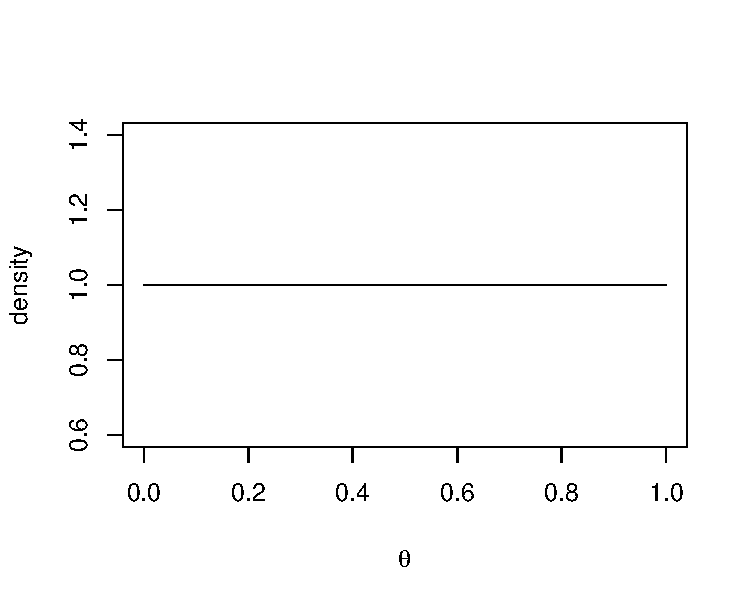
\includegraphics[width = .8\textwidth]{unif.pdf}
\caption{Unif(0,1) prior on $\theta.$}
\label{fig:unif}
\end{figure}
}

\frame{

What happens if we consider though the transformation to $\phi = \dfrac{1}{\theta}.$ 
\vskip 1em
\textcolor{blue}{Think we're moving from the variance to the precision!}

\begin{align}
\phi &= \frac{1}{\theta} \implies 
\theta = \frac{1}{\phi}.
\end{align}

Then using  \textcolor{blue}{\href{https://www.youtube.com/watch?v=lCKxeRiBdjQ}{a change of variables transformation}},
\begin{align}
|\frac{\partial \theta}{\partial \phi}|
& =\frac{1}{\phi^2}.
\end{align}
}

\frame{

\begin{figure}[htdp]
\centering
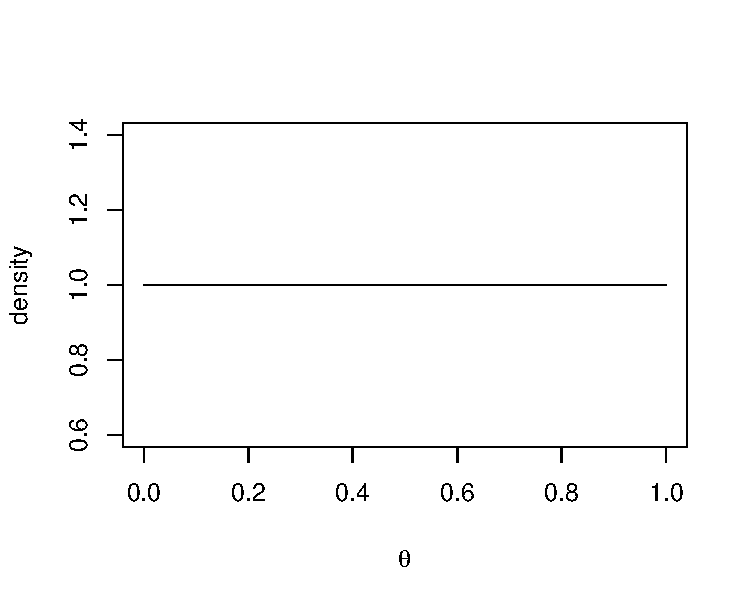
\includegraphics[width = .5\textwidth]{unif.pdf}
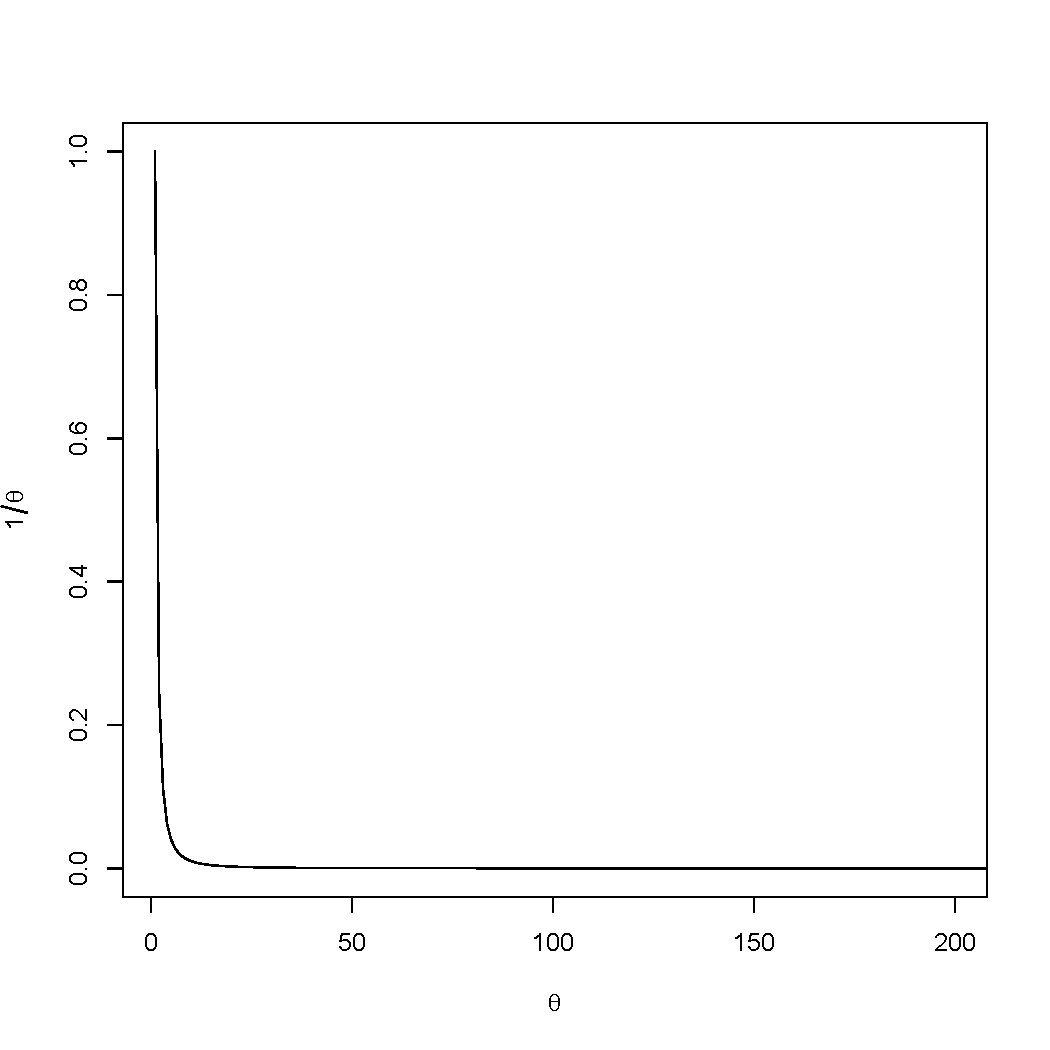
\includegraphics[width = .5\textwidth]{transformationPlot}
\caption{Comparison of the Uniform prior and the transformed prior on $\theta$.}
\label{fig:unif}
\end{figure}


}

\frame{
\frametitle{Recall Jeffrey's prior}

%Exercise: show that Jeffreys' prior is invariant to one-to-one transformations. 

\vskip 1 em

Let's go back over Jeffreys' when $X \sim \text{Bin}(n, \theta).$

\vskip 1 em

How do we calculate Jeffreys' prior?

\vskip 1 em

Specifically, we showed that 
$$p_J(\theta) \propto \text{Beta}(1/2, 1/2).$$

}

\frame{
\frametitle{Recall Jeffrey's prior}

%Exercise: show that Jeffreys' prior is invariant to one-to-one transformations. 



Recall $$p_J(\theta) = \sqrt{\frac{n}{\theta(1-\theta)}}.$$

What happens if we consider though the transformation to $\phi = \dfrac{1}{\theta}?$ 

%
\begin{align}
p_J(\phi) &= p_J(1/\phi) \times |\frac{\partial \theta}{\partial \phi}| \\
& = \sqrt{\frac{n}{ \frac{1}{\phi} (1- \frac{1}{\phi})}} \times \frac{1}{\phi^2}\\
& \propto \frac{\phi} {\sqrt{\phi - 1}}  \times \frac{1}{\phi^2} \\
& \propto \frac{1}{\phi \sqrt{\phi-1}},  \;\;\text{where} \; \;  1 \leq \phi < \infty.
\end{align}
Is the resulting transformation invariant? Yes! 

It's invariant because $\phi = \dfrac{1}{\theta}$ is a one-to-one function.
}

%\frame{
%\frametitle{Is the transformation invariant?}
%Our transformed density $p_J(\phi)$ is \textbf{not in the form of a Beta}, meaning the distribution is not of the ``same form", hence, this transformation is not invariant. \\
%\vskip 1em
%%This should make sense. Why?
%%\vskip 1em
%%The transformation $\phi = 1/\theta$ is not a monotone transformation. (Monotone transformations and Jeffreys' priors are always invariant).
%%\vskip 1em
%%What would be an invariant transformation in this situation? 
%
%
%}

\frame{
Now consider the transformation $\theta = \frac{1}{\sqrt{\phi}}.$

\begin{align}
|\frac{\partial \theta}{\partial \phi}|
& =\frac{1}{2\phi^{3/2}}.
\end{align}

\begin{align}
p_J(1/\sqrt{\phi}) &= p_J(1/\sqrt{\phi}) \times |\frac{\partial \theta}{\partial \phi}| \\
& = (\phi)^{-1/4}
\left(\frac{
\phi^{1/2}-1
}
{\phi^{1/2}
}
\right)^{-1/2}
\times
\frac{1}{2\phi^{3/2}}\\
& \propto  \phi^{3/2} (\phi^{1/2}-1)^{-1/2}
 \;\;\text{where} \; \;  1 \leq \phi < \infty.
\end{align}

Is the resulting transformation invariant? Why or why not? 
(It's also invariant because the transformation is a one-to-one function).

%\vskip 1 em
%If you want to see a proof why this is tru
%Extra reading: \url{https://www2.stat.duke.edu/courses/Fall11/sta114/jeffreys.pdf}
%}
}

\frame{
\frametitle{Take home message with Jeffreys'}
Consider parameter $\theta$ and transformation $g(\theta).$
\vskip 1 em

Jeffreys' prior is invariant under parameterization means that Jeffreys' prior
corresponds to $g(\theta)$ is the \emph{same} as applying a change of ``measure"
or distribution to the Jeffreys' prior for $\theta. $

\vskip 1 em
Said differently, if $\theta = g(\theta),$ then 1 and 2 are the same below.  Let $J$ represent a Jeffreys' prior.

\begin{enumerate}
\item $$J_{\phi} = J_{\theta} \times |\frac{\partial g^{-1}(\theta)}{\partial \theta}| $$
\item $$J_\phi = \sqrt { I(\phi) },$$ 
\end{enumerate} 
where
$I(\phi)$ is the Fisher information of $\phi.$
\vskip 1 em
The proof of this is omitted. (I will post it time permitting).\footnote{Slides 10--13 will not be on midterm 1. You may be asked about other slides or easier questions about objective Bayes and invariance.}


}


% Possibly some things to look at
%http://web.as.uky.edu/statistics/users/pbreheny/701/S13/notes/1-15.pdf


%\frame{
%
%Jeffreys' prior is invariant since we get the same form of the density for $\theta$ and $\phi.$
%\vskip 1 em
%
%The uniform is not invariant to transformations, while Jeffreys' is not. 
%
%\vskip 1 em
%
%This is one reason why Jeffreys' is preferred. 
%
%
%}
%
%\frame{
%
%\begin{figure}[htdp]
%\centering
%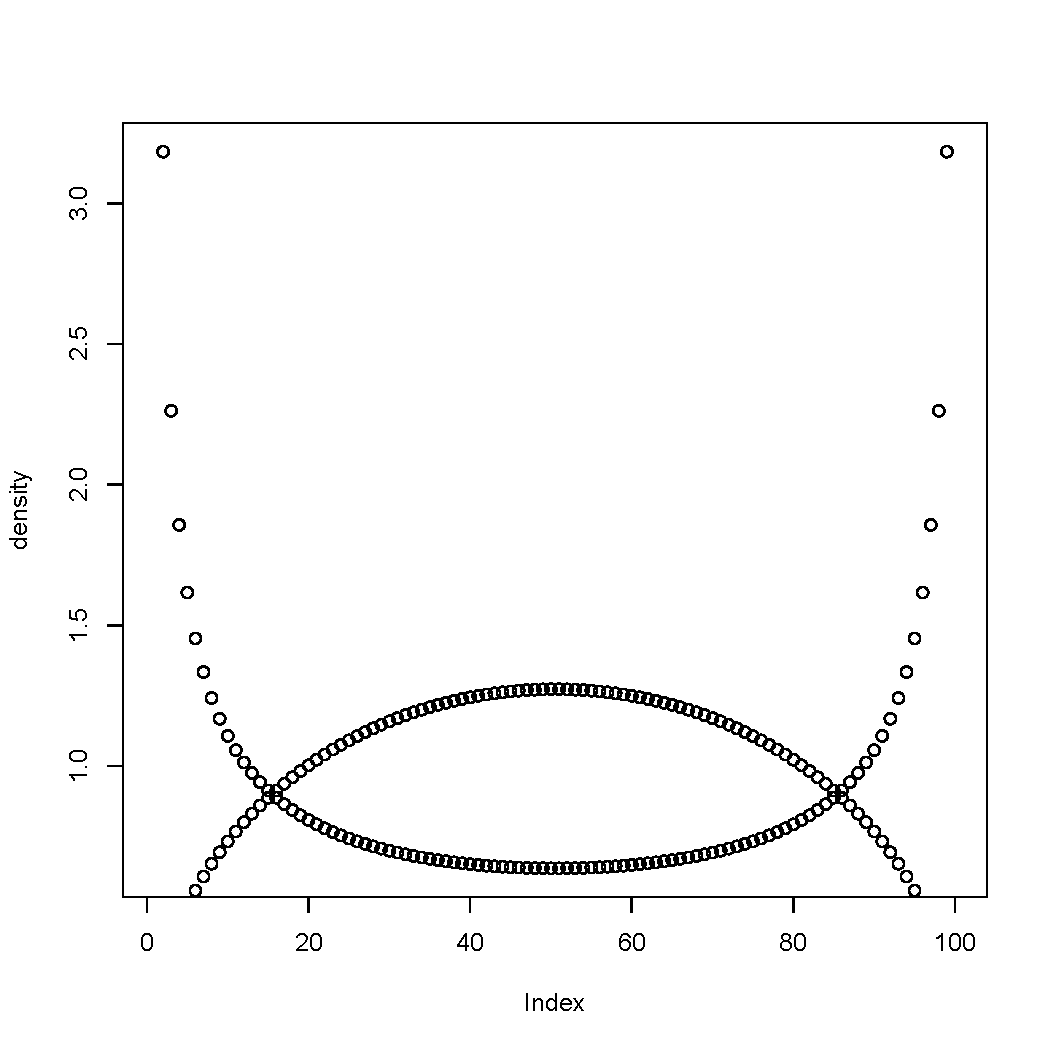
\includegraphics[width = .7\textwidth]{betaInvariant}
%\caption{Beta(1/2,1/2) and Beta(3/2,3/2). Clearly, location invariant.}
%\label{fig:unif}
%\end{figure}
%
%
%}





\end{document}